V tejto semestralnej práci sa budeme venovať problematike v softvérovom inžinierstve a ako zlepšiť život diabetikom po celom svete. S narastajúcim počtom diabetikov po celom svete prevencia už nepostačuje \ref{graf}.

Je potrebné spraviť krok vpred a tím je zaoberanie sa otázkou, ako v dnešnom modernom svete zlepšiť každodenný život diabetikov? 
Táto problematika nemá také ľahké riešenia ako sa zdá. Teória je náročná a riešenia sú v stave testovania.

Na začiatok si povieme čo je diabetes a aké su jeho typy (dva základné). Následne sa pozrieme na niektoré softvérové riešenia ako GIM a alebo Inteligntné riešenie ktoré sú aktuálne testované.
 
\begin{figure}[H]
\centering
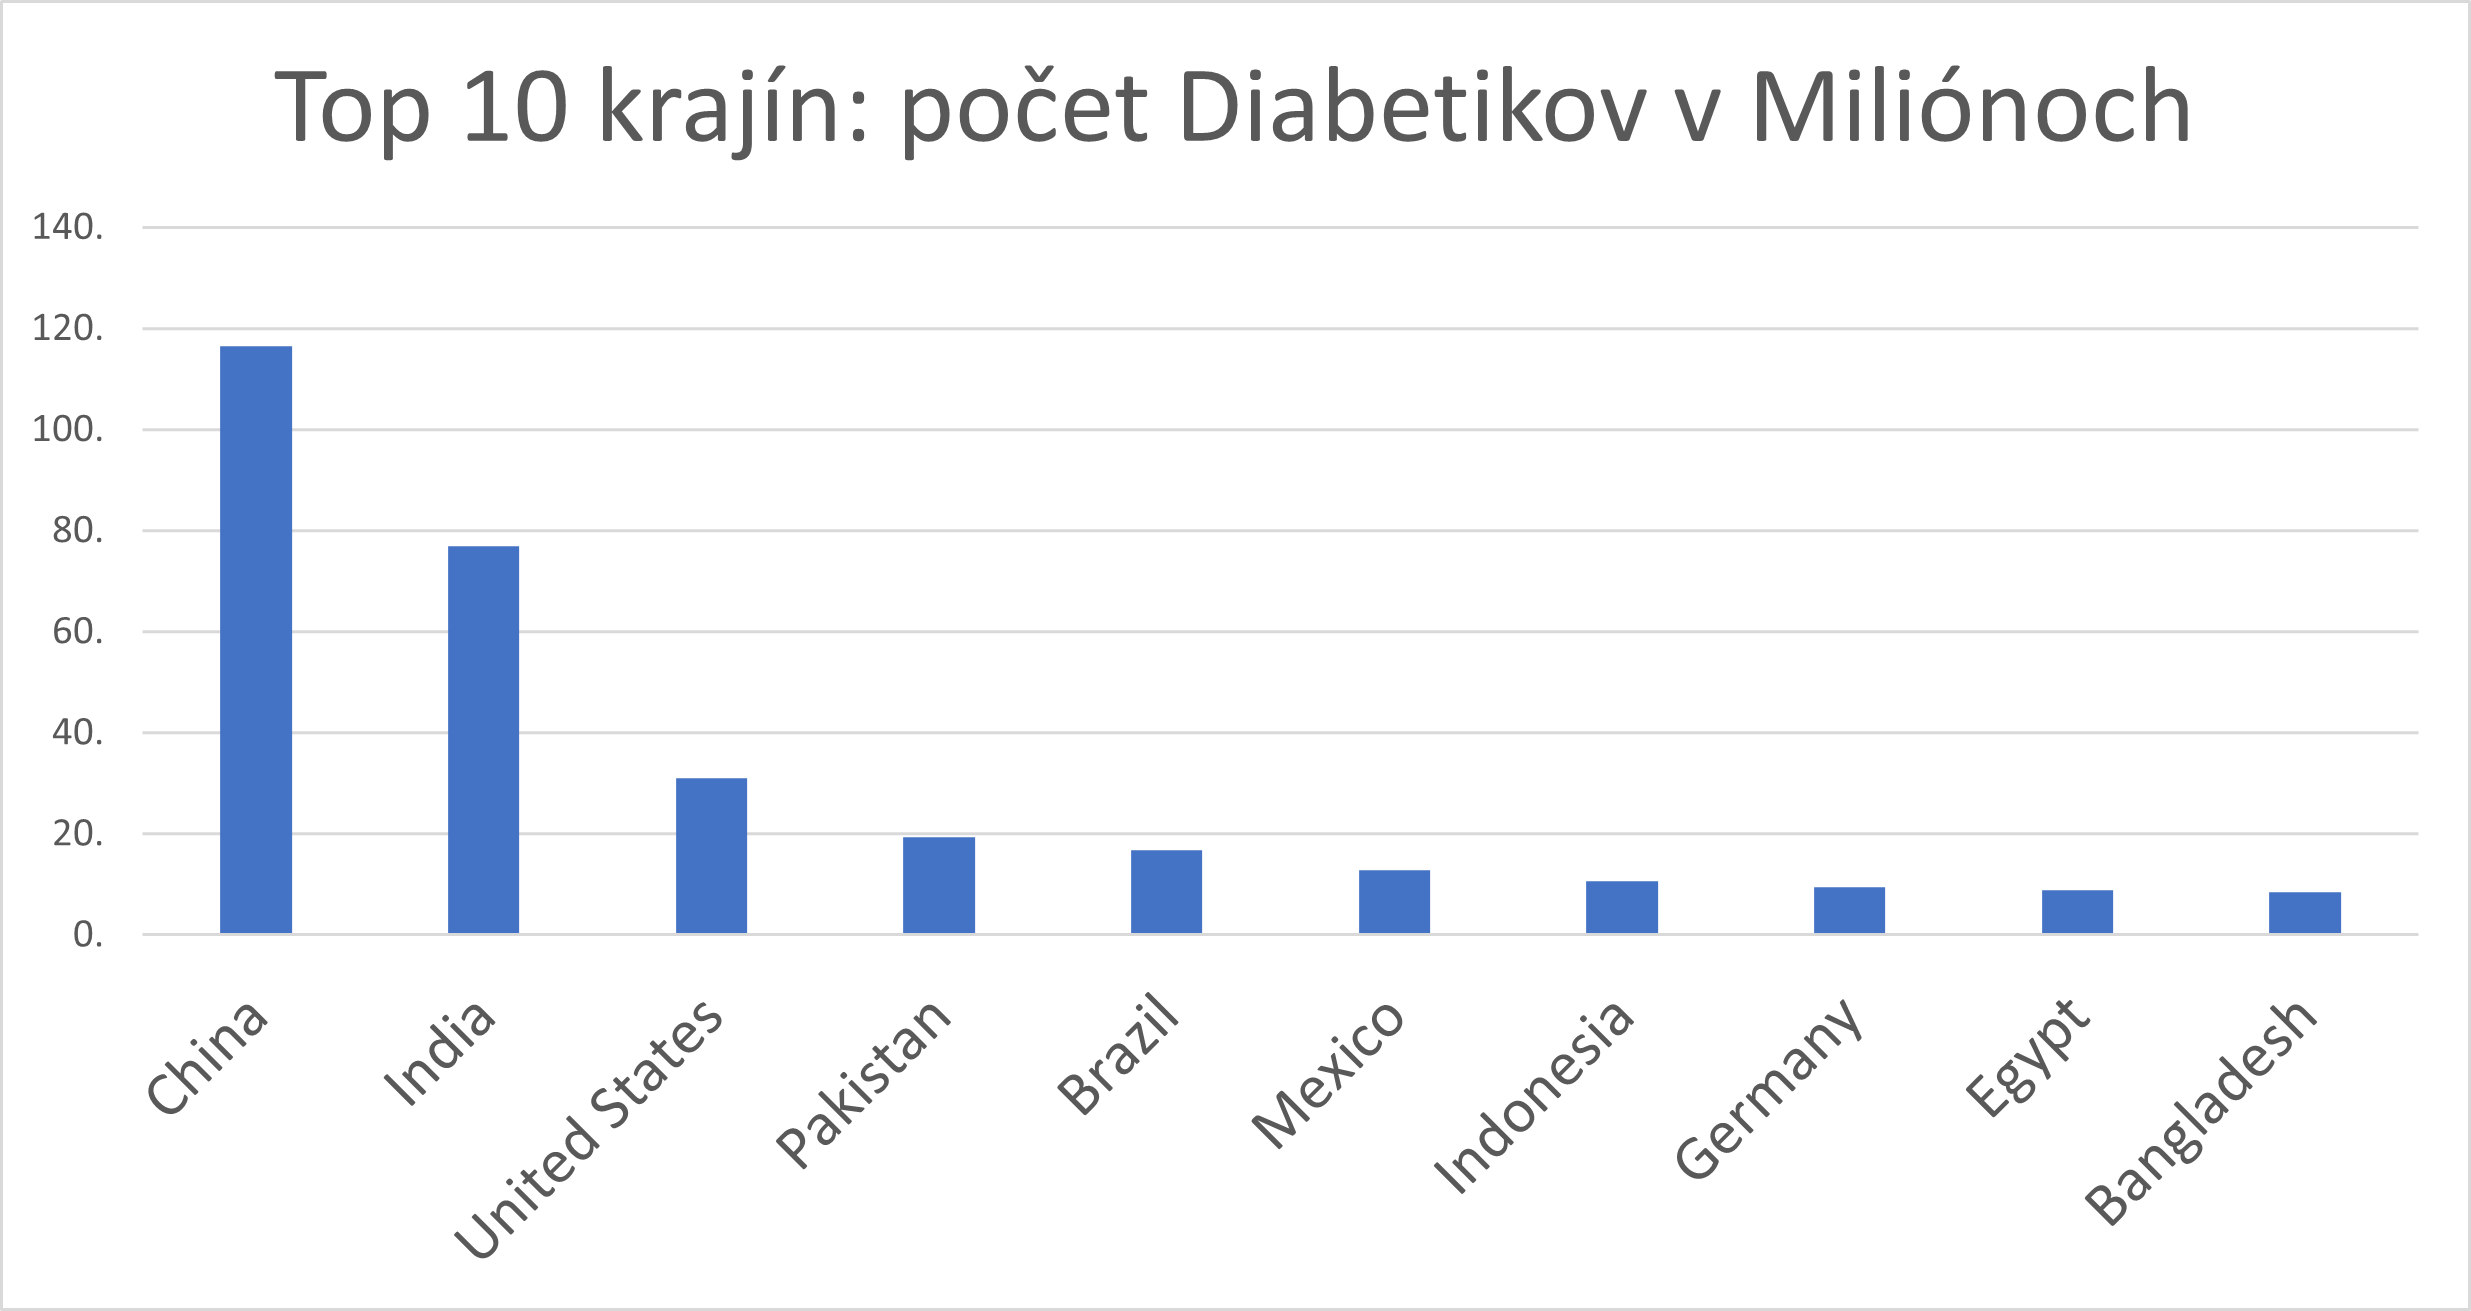
\includegraphics[width=\linewidth]{pocet_diabetikov.png}
\caption{graf znázorňujúci počet diabetikov v miliónoch v roku 2019 \cite{2019s}}
\label{graf}
\end{figure}






